\setcounter{page}{1}

\section{Introducción}
    En las redes de comunicación, la capacidad de capturar y analizar son cosas esenciales para la comprender el comportamiento de los dispositivos y optimizar la comunicación en una red local (LAN). El monitorear y evaluar el tráfico de red puede servirnos al momento de la detección de los problemas de conectividad, diagnosticar algunos fallos en la configuración de los dispositivos que están conectados a la red, de forma que podemos asegurar un flujo eficiente y seguro de los datos.

    Para esta práctica, utilizaremos una herramienta llamada \textbf{Wireshark}  ampliamente usada en el análisis de tráfico en el campo de redes. Wireshark permite capturar y examinar los datos intercambiados entre dos computadores conectados por una (LAN). A través de las capturas, se va a buscar comprender como funcionan los protocolos \textbf{ARP} e \textbf{ICMP} y como estos protocolos nos facilitan la resolución de direcciones y la comunicación entre dispositivos conectados a la red.

    El propósito de esta práctica es el análisis y familiarización con el uso de herramientas como la de Wireshark, para la interpretación de los protocolos ARP y analizar los efectos del comando ping entre dispositivos LAN. Adicionalmente, se busca observar los cambios en la caché ARP tras el intercambio de paquetes y comprender el flujo de tráfico unicast y multicast, así como el intercambio en las estructuras de la red.

    Además de la captura y el análisis de tráfico, es importante entender cómo se comunican los distintos protocolos que conforman la comunicación en redes locales, de manera que interactúen entre sí para garantizar una conectividad eficiente. Tanto el protocolo ARP como el ICMP juegan un papel importante para la resolución de las direcciones así como para la gestión de errores y el diagnostico de problemas de conectividad, como se observa con el uso del comando ping

    A lo largo de este informe, se detallarán los pasos seguidos para la configuración y la captura del tráfico, así mismo, los resultados obtenidos y la interpretación de estos. Este proceso nos permitirá habilidades fundamentales en el análisis del tráfico en la red y en la resolución de problemas que sean comunes en este tipo de redes locales.

\section{Objetivos}
    \begin{itemize}
        \item Emplear la herramienta \textbf{Wireshark} para realizar capturas y análisis de tráfico en una LAN.
        \item Analizar el comportamiento de los mandatos \textbf{ping} en una comunicación vía red.
    \end{itemize}
\section{Marco Teórico}
    Ejemplo de cita~(\cite{buffett84}).

\newpage
\section{Desarrollo del Trabajo}
    \textbf{Para esta práctica se requiere del uso de dos PC's (las denominaremos como PC1 y PC2), ambos equipos conectados por enlace directo y con IP's estáticas.}

    \subsection{Tarea 1.}
        \paragraph{Paso 1.}
        \textbf{Realice una tabla que contenga el nombre de cada equipo, su IP y su MAC.}

        Para comenzar, en la PC1 se inició con el sistema operativo \textbf{Windows} y se realizó el cambio de la dirección IP a \texttt{192.168.0.14} con la puerta de enlace \texttt{192.168.0.1}. Como se muestra en la Figura~\ref{fig:ip_windows}.

        \begin{figure}[H]
            \centering
            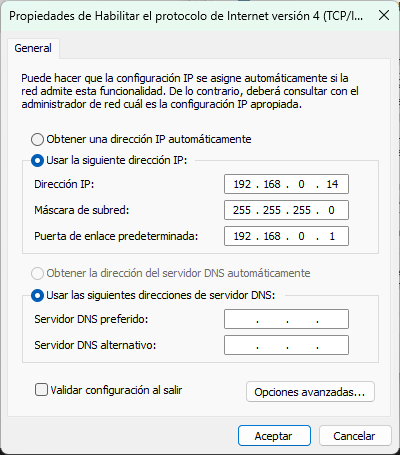
\includegraphics[width=0.6\textwidth]{img/cambiar_IP_Windows.png}
            \caption{Configuración de la Dirección IP en Windows}
            \label{fig:ip_windows}
        \end{figure}

        Para obtener la dirección MAC de un equipo en Windows abrimos la terminal y ejecutamos el comando \texttt{ipconfig -all} y se mostrará la dirección MAC como se muestra en la Figura~\ref{fig:mac_windows}. La dirección MAC que se obtuvo de la PC1 fue \texttt{64:00:6A:44:B6:0A}.

        \begin{figure}[H]
            \centering
            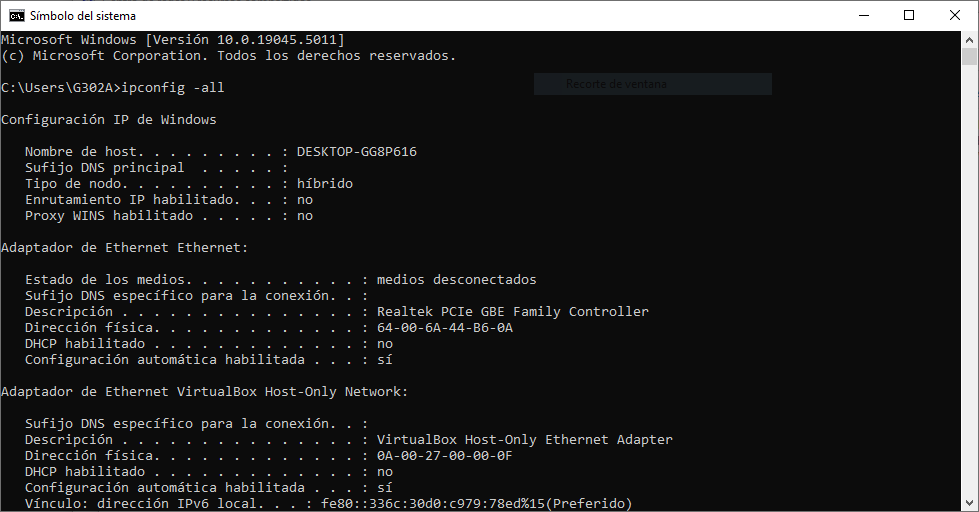
\includegraphics[width=0.6\textwidth]{img/direccion_MAC_windows.PNG}
            \caption{Obtención de la Dirección MAC en Windows}
            \label{fig:mac_windows}
        \end{figure}

        En la PC2 se inició con el sistema operativo \textbf{Linux} y se realizó el cambio de la dirección IP a \texttt{192.168.0.13} con la puerta de enlace \texttt{192.168.0.1}. Como se muestra en la Figura~\ref{fig:ip_linux}.

        \begin{figure}[H]
            \centering
            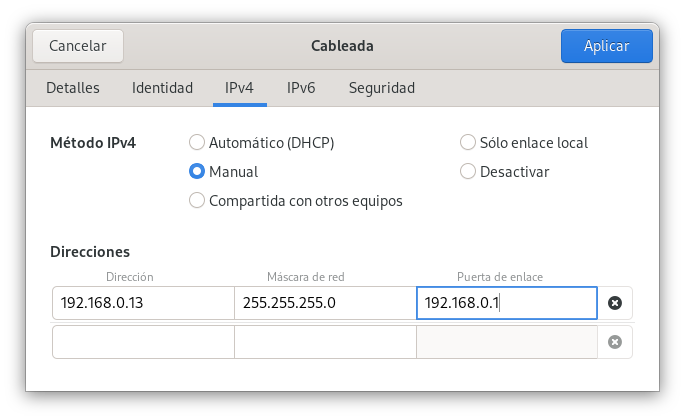
\includegraphics[width=0.6\textwidth]{img/cambiar_IP_Linux.png}
            \caption{Configuración de la Dirección IP en Linux}
            \label{fig:ip_linux}
        \end{figure}
        
        Para obtener la dirección MAC en la PC2 con Linux nos dirigimos a configuración de red y seleccionamos la interfaz de red deseada, en este caso \textbf{Ethernet} y se mostrará la dirección MAC como se muestra en la Figura~\ref{fig:mac_linux}. La dirección MAC que se obtuvo de la PC2 fue \texttt{64:00:6A:44:A5:DF}.
        \begin{figure}[H]
            \centering
            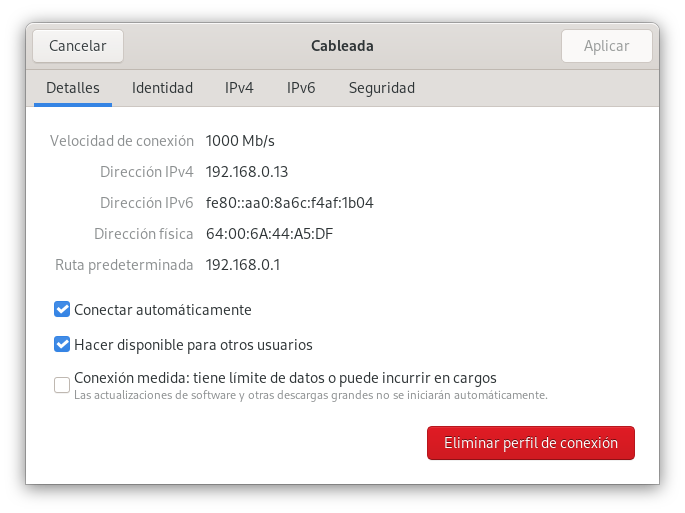
\includegraphics[width=0.6\textwidth]{img/direccion_MAC_linux.png}
            \caption{Obtención de la Dirección MAC en Linux}
            \label{fig:mac_linux}
        \end{figure}

        Los datos obtenidos de ambas PC's se muestran en el Cuadro~\ref{tab:tabla_equipos}.

        \begin{table}[H]
            \centering
            \begin{tabular}{c|c|c|c}
                \textbf{Integrante} & \textbf{Equipo} & \textbf{IP} & \textbf{MAC} \\
                \hline
                Diego Alexis Moreno Valero & PC1 & 192.168.0.14 & 64:00:6A:44:B6:0A \\
                Luis Ángel Cruz Díaz & PC2 & 192.168.0.13 & 64:00:6A:44:A5:DF \\
            \end{tabular}
            \caption{Tabla de Equipos}
            \label{tab:tabla_equipos}
        \end{table}
    \subsection{Tarea 2.}
        \paragraph{Paso 1.}
        Tabla ARP.
        \begin{enumerate}
            \item \textbf{Borre el contenido de la tabla ARP.}\\
            Para borrar la tabla ARP de la PC1, debemos abrir la terminal de Windows y ejecutamos el comando \texttt{arp -d} como se muestra en la Figura~\ref{fig:borrar_arp}. No se muestra la ejecución del comando ya que no se obtiene una respuesta del sistema.
            \begin{figure}[H]
                \centering
                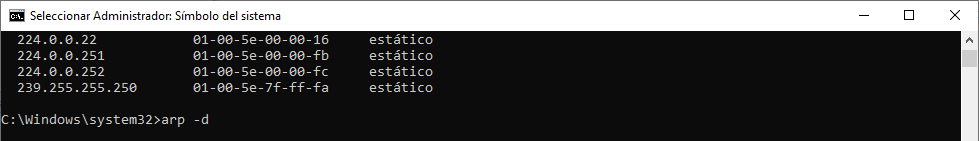
\includegraphics[width=0.6\textwidth]{img/borrar_tabla_ARP.PNG}
                \caption{Borrar Tabla ARP}
                \label{fig:borrar_arp}
            \end{figure}
            \item \textbf{Muestre el contenido de la tabla ARP.}\\
            Para mostrar la tabla ARP de la PC1, debemos abrir la terminal de Windows y ejecutamos el comando \texttt{arp -a} como se muestra en la Figura~\ref{fig:tabla_arp}.
            \begin{figure}[H]
                \centering
                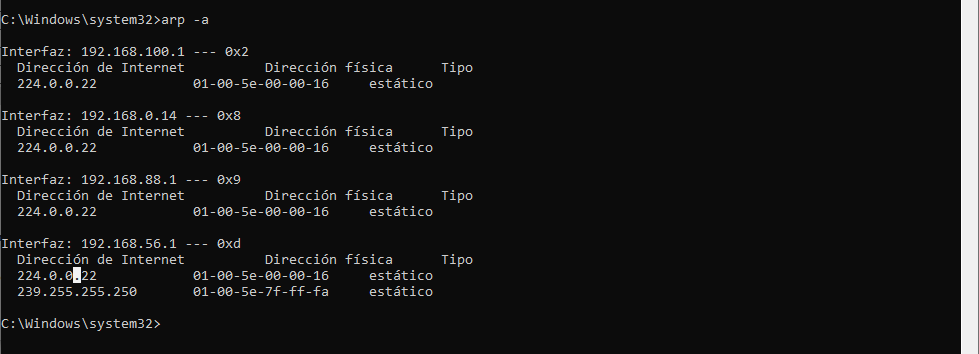
\includegraphics[width=0.6\textwidth]{img/tabla_ARP.PNG}
                \caption{Tabla ARP}
                \label{fig:tabla_arp}
            \end{figure}
            \item \textbf{¿Qué comandos y qué parametros se empleó en los puntos (a) y (b)?}
            \begin{enumerate}
                \item En el punto (a) se empleó el comando \texttt{arp} con el parámetro \texttt{-d} para borrar la tabla ARP. 
                \item En el punto (b) se empleó el comando \texttt{arp} con el parámetro \texttt{-a} para mostrar la tabla ARP.
            \end{enumerate}
            \item \textbf{Explique con detalle el contenido de la tabla.}
            La tabla ARP muestra las direcciones IP y las direcciones físicas (MAC) que están asignadas en el sistema. En esta tabla, se observan varias interfaces (192.168.100.1, 192.168.0.14, 192.168.88.1 y 192.168.56.1), lo cual indica que el dispositivo cuenta con múltiples conexiones de red o adaptadores.
            
            Las direcciones IP presentadas corresponden a los dispositivos en la red con los cuales el dispositivo local ha interactuado o se ha comunicado recientemente. Todas las entradas de la tabla ARP son de tipo \textbf{estático}, lo que significa que estas asociaciones entre direcciones IP y MAC fueron configuradas manualmente o están asignadas de forma permanente, en lugar de ser asignadas dinámicamente por el sistema operativo.
            
            Asimismo, en esta tabla se incluyen direcciones IP de tipo multicast (como 224.0.0.22 y 239.255.255.250), las cuales están asociadas a direcciones MAC específicas. Esto permite que determinados servicios o protocolos de red funcionen correctamente.

            
        \end{enumerate}
        
    \subsection{Tarea 3.}
    \paragraph{Paso 1.}
    Arranquen en la PC1 \textbf{Wireshark} para capturar el tráfico en su interfaz ethernet empleando los filtros adeacuados (ARP).
    \paragraph{Paso 2.}
    Realice el ping de la PC2 a la PC1.
    \begin{enumerate}
        \item ¿Cuál es el comando y los parámetros empleados?\\
        Una vez terminado el ping, interrumpan la captural del Wireshark y guarde la captura en un archivo (utilicen como nombre del archivo captura1.cap)
        Compruebe el estado de las cachés del ARP en la PC.
        \item Consulte la tabla ARP y analice si hubo cambios con los valores obtenidos en el paso 1 de la tarea 2; explique el contenido de la tabla.
    \end{enumerate}
    \paragraph{Paso 3.}
    Configure los filtros para capturar toda la información que se genere. Envíe el ping de la PC2 a la PC1 y al finalizar guarde el archivo como captura2.cap.
    \subsection{Tarea 4.}
    \paragraph{Paso 1.}
    Con Wireshark cargue cada archivo capturado y explique los resultados obtenidos.
    \begin{enumerate}
        \item los campos Ethernet y ARP (peticion y respuesta; archivo: captura)
        \item ICMP(peticion y respuesta; archivos: captura2)
    \end{enumerate}
    
    \section{Conclusiones}
    
    % --- Para agregar un apéndice
    %\newpage
%\appendix
%\appendixpage
%\addappheadtotoc
%\section{Nombre del apéndice}